
\noindent Referring to Figure~\ref{fig:russian-dolls}:

\begin{theorem}
Recursive calculation of the second Brocard triangle produces an infinite sequence of Brocard porisms $\B',\B'',\B''',...$ such that:
\begin{itemize}
    \item The isodynamic points are stationary at the original $X_{15}$ and $X_{16}$.
\item The Brocard circle of each new porism is contained within the Brocard circle of its parent, forming an infinite nesting.
\item Both the circumradius $R$ and the eccentricity $\varepsilon$ of the inellipse decrease monotonically.
\item The Brocard angle $\omega$ increases monotonically and converges to $\pi/6$ (i.e., triangles approach equilaterals).
\item The sequence of porisms converges to $X_{15}$.
\end{itemize}
\label{thm:nesting}
\end{theorem}

\begin{proof}
Corollary~\ref{cor:x15x16p} entails fixed isodynamic points. Proposition~\ref{prop:containment} entails Brocard circle infinite nesting. The other results stem from recursive application of relations in Theorem~\ref{thm:porism}.
\end{proof}

\noindent Defined in \cite[p. 78]{morley54}, and cited in  \cite[P(2)]{etc-bicentric}:

\begin{definition}[Beltrami Points]
Denoted $P_2$ and $U_2$, these are the inverses with respect to the circumcircle of the Brocard points. They lie on the Beltrami (or Lemoine) axis $L_{563}$, parallel to a line through the Brocard points \cite[Central Lines]{etc}.
\end{definition}

\noindent Introduced in \cite{gibert2020-anti-brocard}:

\begin{definition}(Anti second Brocard triangle)
Given a triangle $T$, its anti second Brocard triangle $T^*$ is a triangle whose second Brocard is $T$. 
\end{definition}

\begin{proposition}
Recursive calculation of the anti second Brocard triangle produces an infinite sequence of Brocard porisms $\B^*,\B^{**},\B^{***},...$ such that:
\begin{itemize}
    \item The isodynamic points remain stationary at the original $X_{15}$ and $X_{16}$.
\item The Brocard circle of each new porism is exterior to the previous one, forming a reverse infinite nesting.
\item The sequence of porisms converges to segment $P_2 U_2$, i.e:
\begin{itemize}
\item The inellipse major (resp. minor) semi-axis converges to $|P_2 U_2|$ (resp. 0).
\item The circumradius $R$ monotonically increases and converges to infinity.
%$|P(2)U(2)|$
\item The Brocard angle $\omega$ decreases monotonically to zero.
\end{itemize}
\end{itemize}
\label{prop:anti-nesting}
\end{proposition}

\begin{proof}
The result follows applying Theorem \ref{thm:porism}  and Propositions \ref{prop:orbita} and \ref{prop:conjunto_limite}  observing that we can invert the process of recurrence taking the sequence of second anti Brocard triangles  $T^*$, $T^{**},\ldots,$ as   isosceles triangles tangent to the Brocard innelipse as shown in Fig. \ref{fig:russian-dolls-10}.
\end{proof}

\begin{definition}[Beltrami Circles]
Given a triangle, let $\Cm_1$ (resp. $\Cm_2$) denote the first (resp. second) Beltrami circle, passing through the first $P_2$ (resp. second $U_2$) Beltrami point, containing their circumcircle inverse $\Omega_1$ (resp. $\Omega_2$).
\end{definition}

\begin{lemma} The the Beltrami circles $\Cm_1$ and $\Cm_2$ are centered on
\[ P_2,U_2=\left[\mp\frac{R}{\sqrt{\Sha^2-3}}, -\frac{R\Sha}{\sqrt{\Sha^2-3}}\right]
\]
\label{lem:beltrami}
\end{lemma}
\begin{proof} The circumcircle inverse of $\Omega_1$ is $O_1=P_2$ and that of $\Omega_2$ is $O_2=U_2$. 
Therefere, 
\[P_2=R^2\frac{\Omega_1}{|\Omega_1|^2},\;\;\; U_2=R^2\frac{\Omega_2}{|\Omega_2|^2}\]
Therefore the result follows from Proposition \ref{prop:brocs12}. 

\end{proof}

\begin{proposition}\label{prop:beltrami_circles}
The Beltrami circles intersect at $X_{15}$ and $X_{16}$ and their radii $\rho$ is equal and given by:
\[ \rho = \frac{2R}{\sqrt{\Sha^2-3}}\] 
Moreover, the triangles $X_{15} P_2 U_2$ and $X_{16} P_2 U_2$ are equilateral.
\end{proposition}

\begin{proof} Follows from Lemmas \ref{lem:x15x16} and \ref{lem:beltrami}.
\end{proof}

\begin{theorem}
The sequence $\Omega_1$, $\Omega_2'$, ${\Omega_1}''$, ${\Omega_2}'''$, etc. (resp. $\Omega_2$, $\Omega_1'$, ${\Omega_2}'''$, ${\Omega_1}'''$) is concyclic on the first (resp. second) Beltrami circle.
\label{thm:concyclic}
\end{theorem}

\begin{proof} Using Proposition  \ref{prop:orbita}, Lemma \ref{lem:reciprocal}  and Theorem \ref{thm:porism} we compute explicitly the sequence of   Brocrard points stated. It is straightforward to derive the equation of the circles. They are given by

\begin{align*}
  \Cm_1 &:  4 h^2 (3 d^2-h^2)  (x^2+y^2) -8 d h^2 \zeta  x  -4 h (3 d^2+h^2) \zeta y+(3 d^2-h^2) \zeta^2=0\\
    \Cm_2 &: 4 h^2 (3 d^2-h^2)  (x^2+y^2) + 8 d h^2 \zeta  x  -4 h (3 d^2+h^2) \zeta y+(3 d^2-h^2) \zeta^2=0\\
\end{align*}

\noindent where $\zeta=d^2+h^2$. The centers are
\[ O_{1,2}= \left[\pm\frac{d \zeta}{3d^2-h^2}, \frac{(3d^2+h^2)\zeta}{ 2h(3d^2-h^2)}\right]=\left[\pm\frac{R}{\sqrt{\Sha^2-3}} ,-\frac{R\Sha}{ \sqrt{\Sha^2-3}}\right]
\] 
The common radius $\rho$ is given by
\[\rho=\frac{2d \zeta}{3d^2-h^2}=
\frac{2R}{\sqrt{\Sha^2-3}}\]
The intersections of $\Cm_1$ and $\Cm_2$ are  triangle centers $X_{15}$, $X_{16}$ of Lemma \ref{lem:x15x16}.
\end{proof}

\noindent Using the definition in \cite[Isodynamic Points]{mw}:

\begin{definition}(Apollonius Circles)
Given a triangle, there are three circles passing through one vertex and both isodynamic points $X_{15}$ and $X_{16}$.
\end{definition}

Let $\T$ be the upright isosceles Ponecelet triangle with half base $d$ and height $h$.

\begin{corollary}
The Beltrami circles are the first and second Apollonius circles of $\T$. The third Apollonius circle is degenerate and coincides with the Brocard axis.
\end{corollary}

\begin{proof}
The anti-second Brocard $\T^*$ of $\T$ has Brocard points $\Omega_2^*,\Omega_1^*$ which coincide with vertices $B$ and $A$ of $\T$. Applying Theorem~\ref{thm:concyclic} in reverse direction, $\Omega_2^*,\Omega_1^*$ will lie each on $\Cm_2$ and $\Cm_1$, respectively. Therefore $\Cm_2$ (resp. $\Cm_1$) passes through vertex $B$ (resp. $A$) and the two stationary isodynamic points $X_{15}$, $X_{16}$ (anti-Brocards preserve these). By definition these are the first and second Apollonius circles \cite[Isodynamic Points]{mw}. The third Apollonius circle contains the two isodynamic points and vertex $C$ of $\T$. Since these are collinear on the Brocard axis, the circle is a line.
\end{proof}


\begin{proposition}
$\Cm_1$ and $\Cm_2$ are perpendicular to each Brocard circle in the sequence.
\end{proposition}
\begin{proof}
It is straightforward to verify the claim for the circumcircle of isosceles triangle $\T$, given implicitly by
\[ x^2+y^2-R^2=0, \;\; R=\frac{d^2+h^2}{2 h}.\]
\end{proof}
\begin{figure}
    \centering
 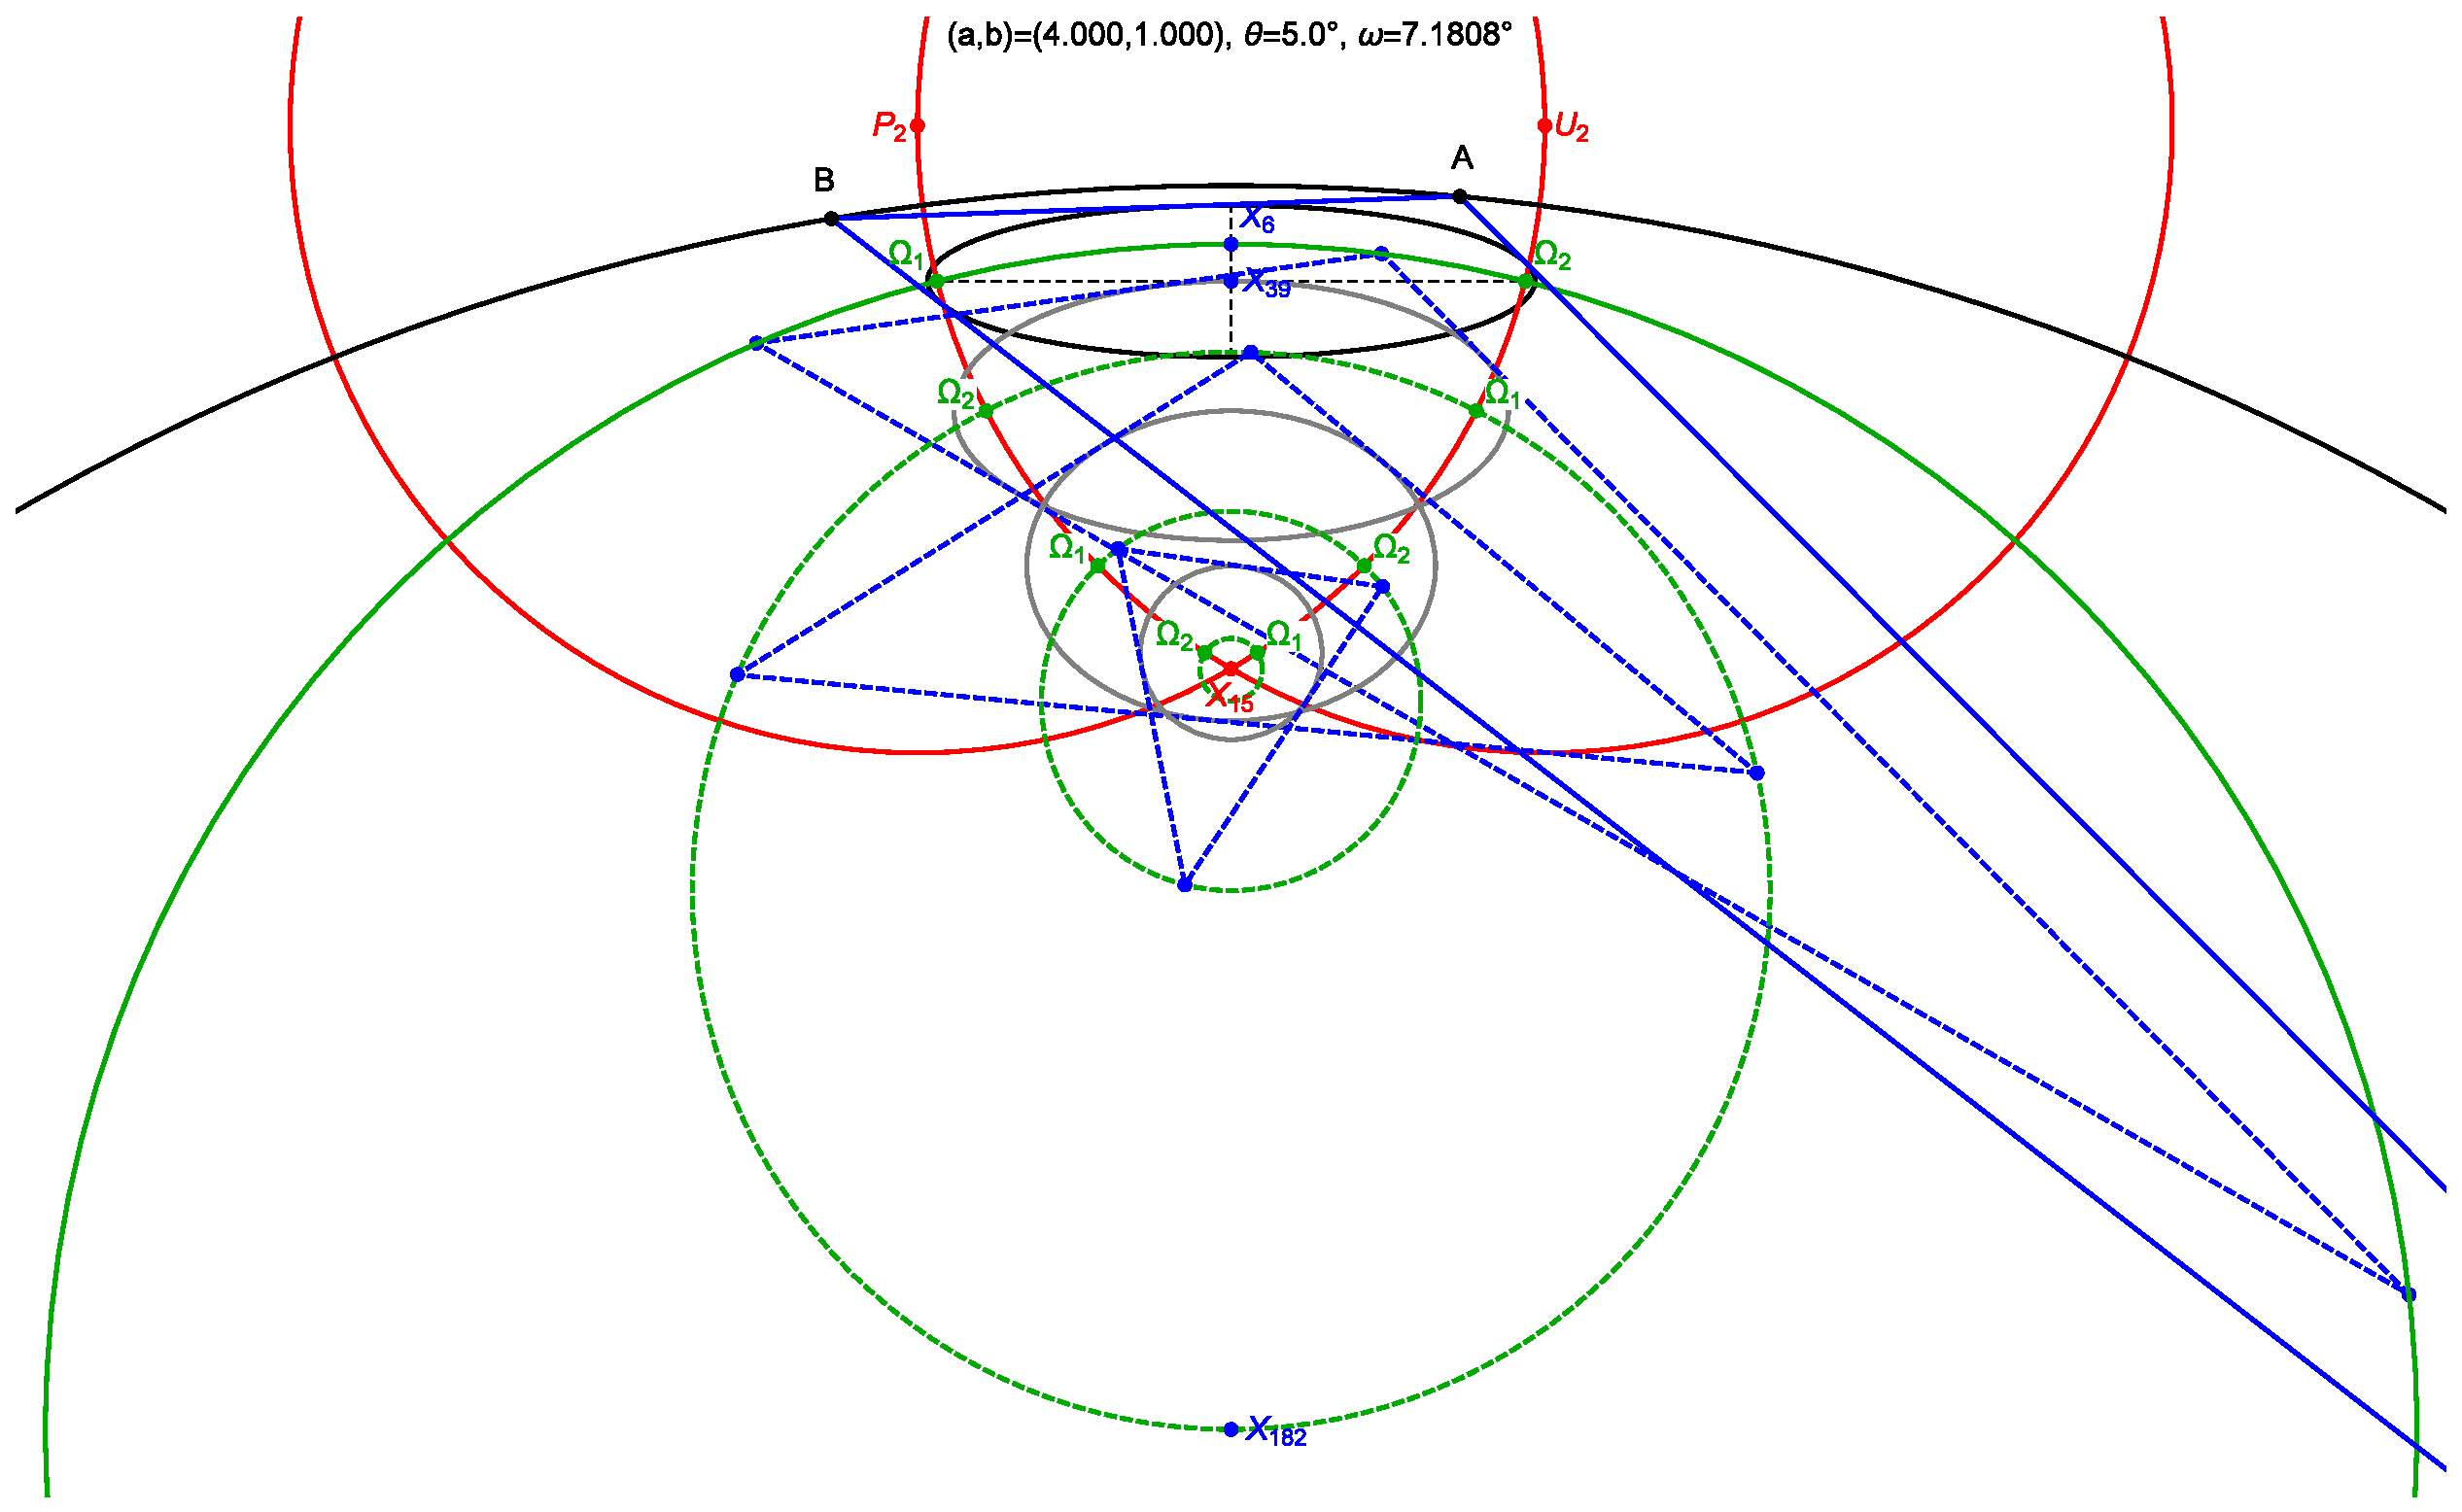
\includegraphics[width=\textwidth]{pics_06_0110_broc_porism_russian_circles.eps}
    \caption{Three iterations of second Brocard triangles (dashed blue), each spawning its own Brocard porism. Successive Brocard points descend in alternate fashion along two circular arcs (red). These intersect at $X_{15}$ and  $X_{16}$ (above page, not shown), with centers on the Beltrami points $P_2,U_2$. The sequence of Brocard points and porisms converges to the first isodynamic point $X_{15}$, common to all porisms. At every generation the circumcircle-inellipse pair approaches a shrinking pair of concentric circles (the triangle family approaches equilaterals).  \href{https://youtu.be/Z3YlEbCFbnA}{Video}}
    \label{fig:russian-dolls}
\end{figure}

\begin{figure}[H]
    \centering
    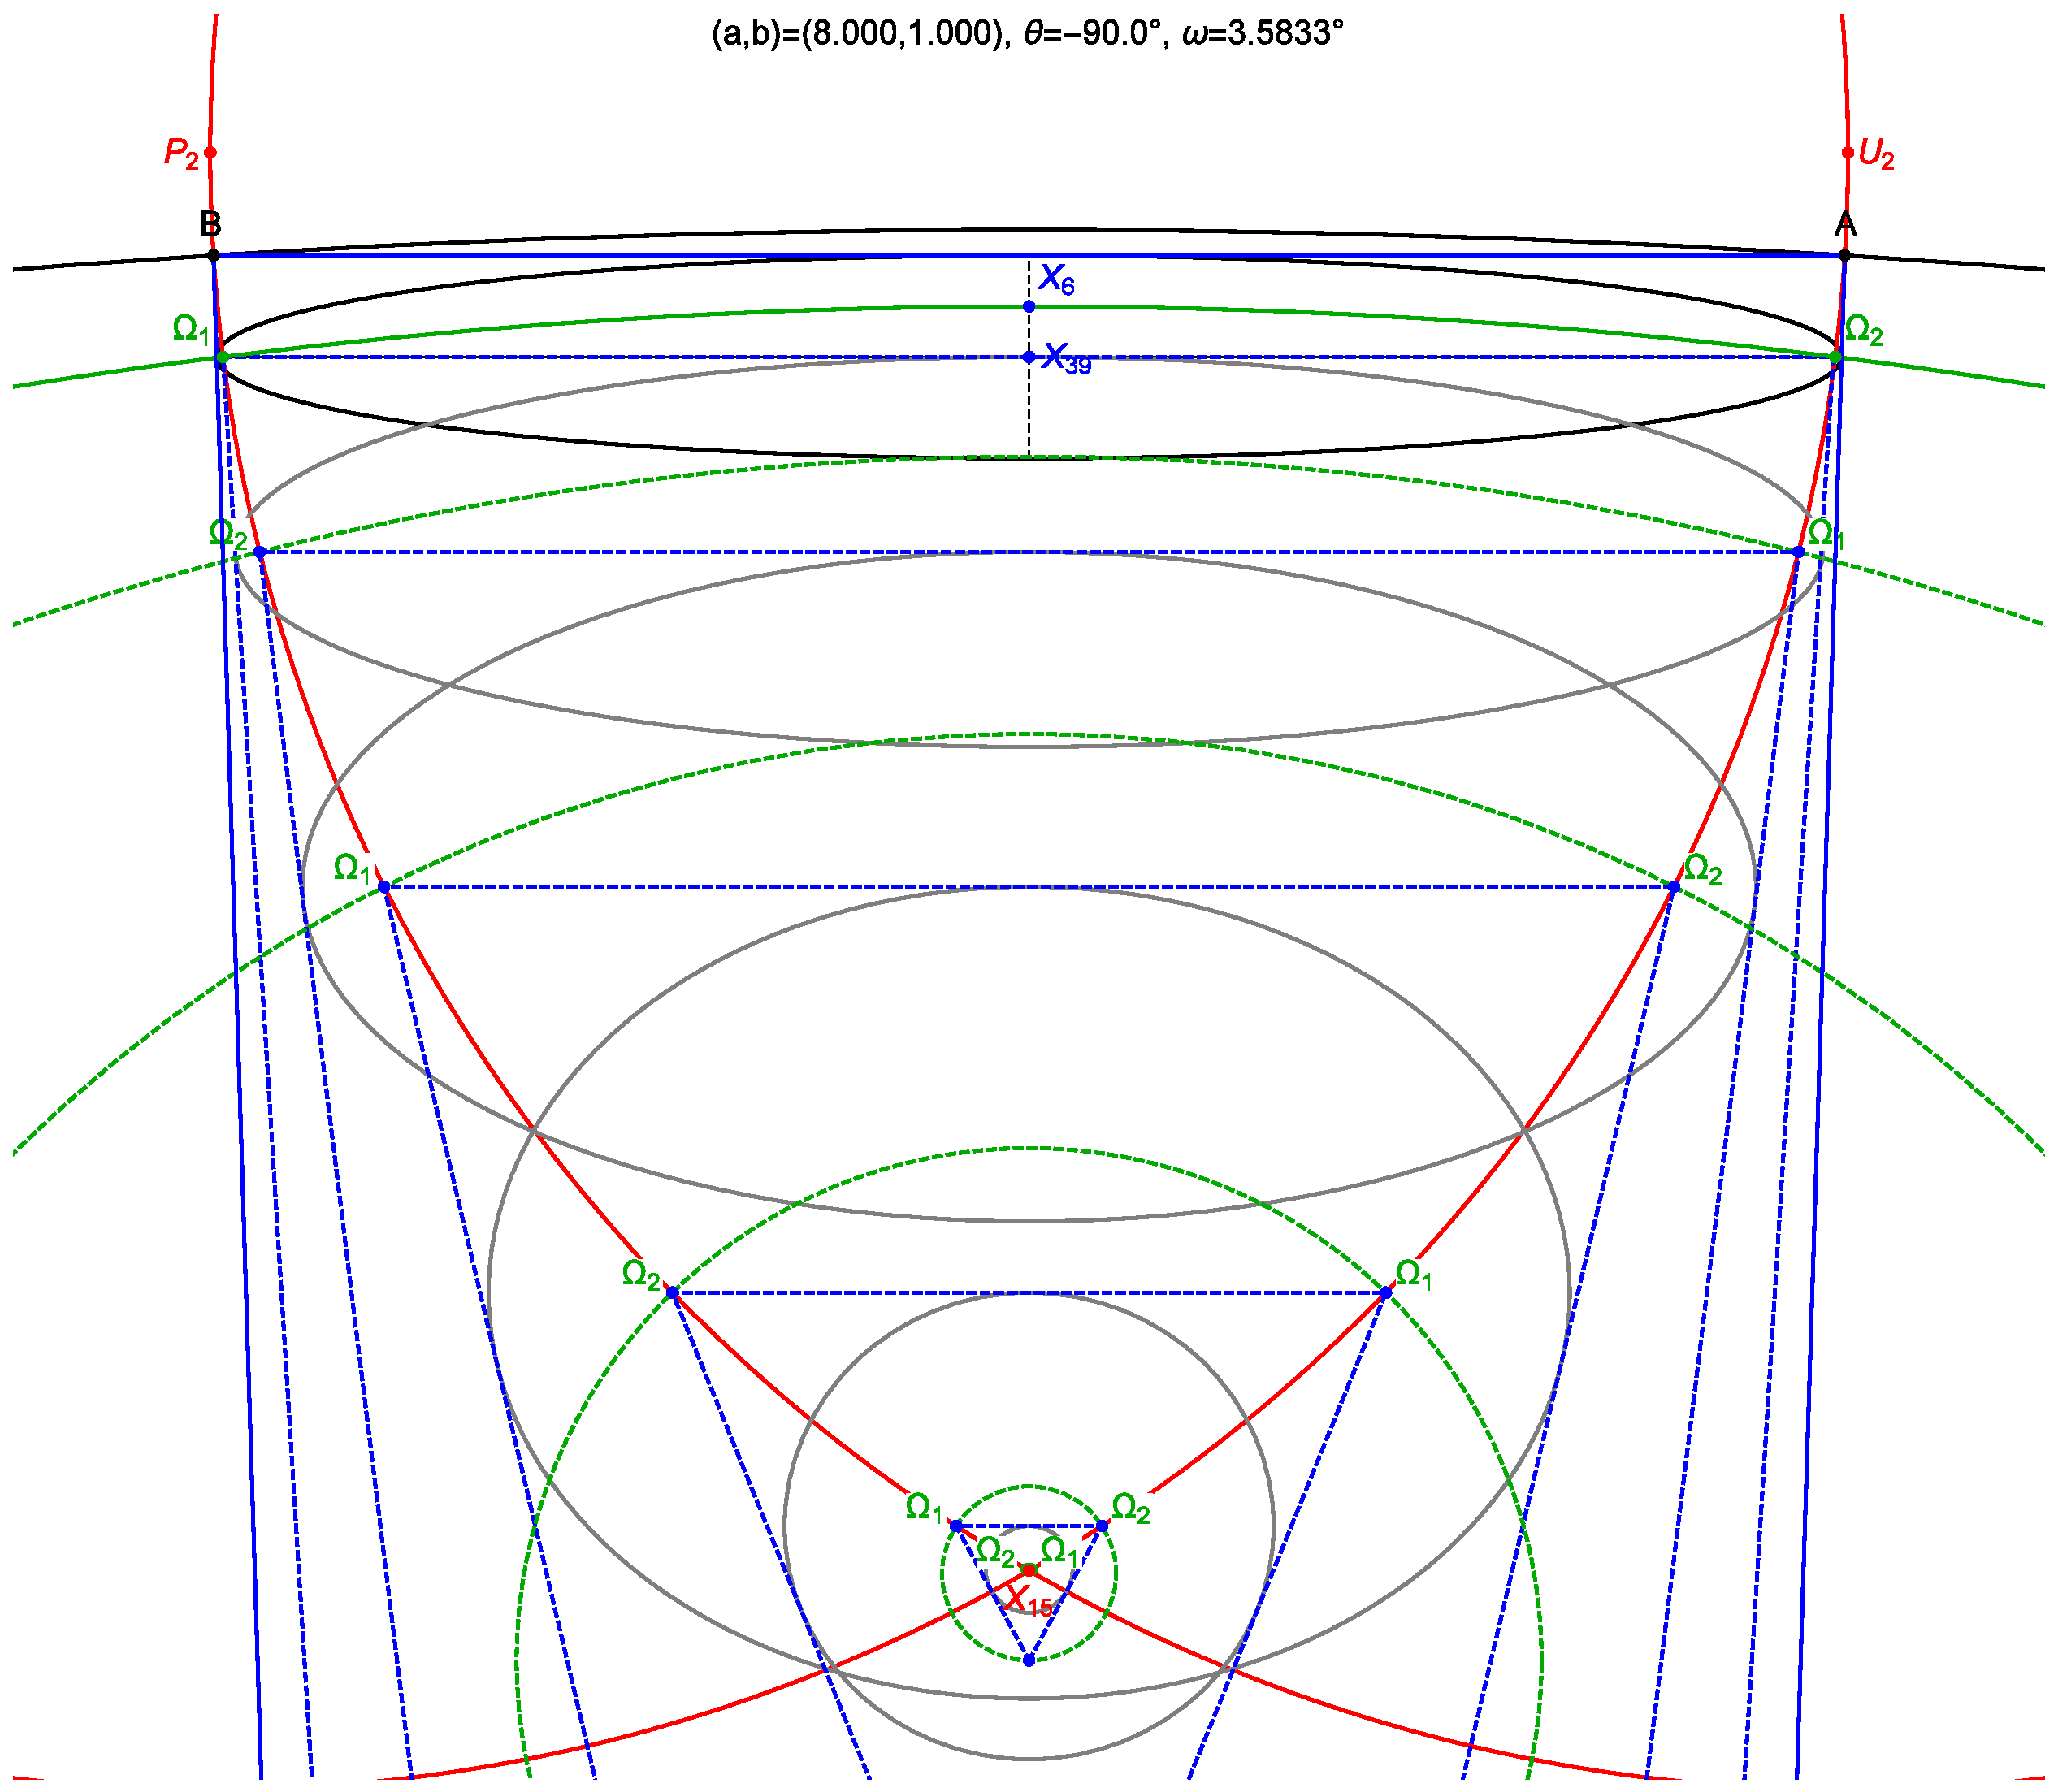
\includegraphics[width=.9\textwidth]{pics_06_0120_broc_porism_russian_circles.eps}
    \caption{Sequence of porisms with successive Brocard points walking along two circular arcs (red) bounded by the Beltrami points $P_2,U_2$ and $X_{15}$. For each generation the isosceles $\T$ Poncelet triangle is shown (solid blue = first generation, dashed blue = subsequent ones). The bottom vertex is not shown (below the page). The base vertices $A,B$, or $A',B'$, etc., of a given $\T$ are the Brocard points of the previous generation. And that their midpoint coincides with the top vertex of the Brocard inellipse.}
    \label{fig:russian-dolls-10}
\end{figure}


